%
% $RCSfile: paper.tex,v $
%
% Copyright (c) 2004. Christian Heller. All rights reserved.
%
% No copying, altering, distribution or any other actions concerning this
% document, except after explicit permission by the author!
% At some later point in time, this document is planned to be put under
% the GNU FDL license. For now, _everything_ is _restricted_ by the author.
%
% http://www.cybop.net
% - Cybernetics Oriented Programming -
%
% http://www.resmedicinae.org
% - Information in Medicine -
%
% @author Christian Heller <christian.heller@tuxtax.de>
%

%
% The document class specifying the type of document.
%
\documentclass[a4paper,10pt]{llncs}

%
% The usepackages for document class.
%

% Paper format and font.
\usepackage{a4,times,helvet}

% Graphics.
\usepackage{graphicx}

%
% The space settings for edges (left, top, right, bottom).
%
\setlength{\hoffset}{-3,9cm}
\setlength{\voffset}{-3,6cm}
\setlength{\oddsidemargin}{4cm}
\setlength{\evensidemargin}{3cm}
\setlength{\topmargin}{1,5cm}
\setlength{\textwidth}{17cm}
\setlength{\textheight}{25cm}

%
% The hyphenation list.
%
%
% $RCSfile: hyphenation.tex,v $
%
% Copyright (c) 2001-2004. Christian Heller. All rights reserved.
%
% No copying, altering, distribution or any other actions concerning this
% document, except after explicit permission by the author!
% At some later point in time, this document is planned to be put under
% the GNU FDL license. For now, _everything_ is _restricted_ by the author.
%
% http://www.cybop.net
% - Cybernetics Oriented Programming -
%
% http://www.resmedicinae.org
% - Information in Medicine -
%
% @author Christian Heller <christian.heller@tuxtax.de>
%

\hyphenation{abs-trac-tion}
\hyphenation{abs-trac-tions}
\hyphenation{ac-tu-ally}
\hyphenation{addi-tio-nally}
\hyphenation{ana-lyst}
\hyphenation{ana-ly-sis}
\hyphenation{an-cient}
\hyphenation{ap-pli-ca-tion}
\hyphenation{arche-types}
\hyphenation{aris-to-tle}
\hyphenation{at-tri-bute}
\hyphenation{avoi-da-ble}
\hyphenation{be-ing}
\hyphenation{binary}
\hyphenation{bran-ches}
\hyphenation{ca-te-go-ri-za-tion}
\hyphenation{client}
\hyphenation{com-po-nen-ti-za-tion}
\hyphenation{com-pu-ter}
\hyphenation{con-fi-gure}
\hyphenation{con-fi-gu-ra-tion}
\hyphenation{con-nec-ted}
\hyphenation{cri-ti-cised}
\hyphenation{cy-ber-ne-tics}
\hyphenation{cyboi}
\hyphenation{cybol}
\hyphenation{cybop}
\hyphenation{de-sign}
\hyphenation{des-cribe}
\hyphenation{des-cribed}
\hyphenation{de-ve-lop-ment}
\hyphenation{dis-crete}
\hyphenation{di-vide}
\hyphenation{do-main}
\hyphenation{dy-na-mic}
\hyphenation{dy-na-mics}
\hyphenation{ela-bo-ra-ted}
\hyphenation{ele-ments}
\hyphenation{en-gi-nee-ring}
\hyphenation{eng-lish}
\hyphenation{en-vi-ron-ment}
\hyphenation{ex-pert}
\hyphenation{fi-gure}
\hyphenation{fun-da-men-tal}
\hyphenation{func-tio-na-li-ty}
\hyphenation{hard-ware}
\hyphenation{hu-man}
\hyphenation{im-ple-men-ta-tion}
\hyphenation{imp-roved}
\hyphenation{in-he-rit}
\hyphenation{in-ter-pre-ter}
\hyphenation{java}
\hyphenation{know-ledge}
\hyphenation{lan-guage}
\hyphenation{li-ving}
\hyphenation{lo-gi-cal}
\hyphenation{machine}
\hyphenation{me-cha-nism}
\hyphenation{me-thods}
\hyphenation{na-ture}
\hyphenation{net-work}
\hyphenation{neu-ral}
\hyphenation{neu-ron}
\hyphenation{nu-me-rous}
\hyphenation{object}
\hyphenation{open}
\hyphenation{operating}
\hyphenation{ori-en-ted}
\hyphenation{over-come}
\hyphenation{prin-ci-ple}
\hyphenation{prin-ting}
\hyphenation{pro-ba-bi-lis-tic}
\hyphenation{pro-gram-ming}
\hyphenation{re-cog-nize}
\hyphenation{re-cog-nized}
\hyphenation{re-pre-sen-ta-tion}
\hyphenation{re-pre-sen-ting}
\hyphenation{re-u-sa-bi-li-ty}
\hyphenation{sci-ence}
\hyphenation{server}
\hyphenation{se-pa-ra-ted}
\hyphenation{se-pa-ra-tion}
\hyphenation{si-mi-lar}
\hyphenation{soft-ware}
\hyphenation{source}
\hyphenation{spe-cia-li-za-tion}
\hyphenation{sta-tic}
\hyphenation{sta-ti-cal-ly}
\hyphenation{sto-chas-tic}
\hyphenation{stone-on-stone}
\hyphenation{struc-ture}
\hyphenation{strug-gling}
\hyphenation{su-per-flu-ous}
\hyphenation{sup-ply-ing}
\hyphenation{sys-tem}
\hyphenation{tes-ting}
\hyphenation{thin-king}
\hyphenation{un-en-li-vened}
\hyphenation{un-fa-vou-ra-ble}
\hyphenation{un-sa-tis-fy-ing}
\hyphenation{va-ry-ing}
\hyphenation{weigh-ted}


%
% This document is a scientific paper to be handed in for a conference.
%
% @version $Revision: 1.3 $ $Date: 2005-03-14 22:21:15 $ $Author: christian $
% @author Christian Heller <christian.heller@tuxtax.de>
% @author Christian Heller <christian.heller@tu-ilmenau.de>
%
\begin{document}
    \twocolumn
    %
% $RCSfile: title.tex,v $
%
% Copyright (c) 2001-2004. Christian Heller. All rights reserved.
%
% No copying, altering, distribution or any other actions concerning this
% document, except after explicit permission by the author!
% At some later point in time, this document is planned to be put under
% the GNU FDL license. For now, _everything_ is _restricted_ by the author.
%
% http://www.cybop.net
% - Cybernetics Oriented Programming -
%
% http://www.resmedicinae.org
% - Information in Medicine -
%
% @author Christian Heller <christian.heller@tuxtax.de>
%

\title{A new Pattern Systematics}
\author{
    Christian Heller \(<\)christian.heller@tu-ilmenau.de\(>\)\\
    Detlef Streitferdt \(<\)detlef.streitferdt@tu-ilmenau.de\(>\)\\
    Ilka Philippow \(<\)ilka.philippow@tu-ilmenau.de\(>\)
}
\institute{Technical University of Ilmenau\\
    Faculty for Computer Science and Automation\\
    Institute for Theoretical and Technical Informatics\\
    PF 100565, Max-Planck-Ring 14, 98693 Ilmenau, Germany\\
    http://www.tu-ilmenau.de, fon: +49-3677-69-1230, fax: +49-3677-69-1220 \vspace*{0.5cm}
}

    \maketitle
    %
% $RCSfile: abstract.tex,v $
%
% Copyright (c) 2001-2004. Christian Heller. All rights reserved.
%
% No copying, altering, distribution or any other actions concerning this
% document, except after explicit permission by the author!
% At some later point in time, this document is planned to be put under
% the GNU FDL license. For now, _everything_ is _restricted_ by the author.
%
% http://www.cybop.net
% - Cybernetics Oriented Programming -
%
% http://www.resmedicinae.org
% - Information in Medicine -
%
% @author Christian Heller <christian.heller@tuxtax.de>
%

\begin{center}
    \textbf{\large{Abstract}}
\end{center}
\normalsize
\textit{
This document describes how existing design patterns can be combined to merge
their advantages into one domain- independent software framework. This framework,
called Cybernetics Oriented Programming (CYBOP), is characterized by flexibility
and extensibility. Further, the concept of Ontology is used to structure the
software architecture as well as to keep it maintainable. A Component Lifecycle
ensures the proper startup and shutdown of any systems built on top of CYBOP.\\
The practical proof of these new concepts was accomplished within the diploma
thesis of Jens Bohl which consisted of designing and developing a module called
Record, of the Open Source Software (OSS) project Res Medicinae. The major task
of this module is to provide a user interface for creating medical documentation.
New structure models such as Episodes were considered and implemented. In this
context, the integration of a graphical tool for Topological Documentation was
also highly demanded. The tool allows documentation with the help of anatomical
images and the setting of markers for pathological findings.\\
\textbf{Keywords.} Design Pattern, Framework, Component Lifecycle, Ontology,
CYBOP, Res Medicinae, Episode Based Documentation, Topological Documentation
} \rm


    %
% $RCSfile: introduction.tex,v $
%
% Copyright (c) 2005-2006. Christian Heller. All rights reserved.
%
% Permission is granted to copy, distribute and/or modify this document
% under the terms of the GNU Free Documentation License, Version 1.1 or
% any later version published by the Free Software Foundation; with no
% Invariant Sections, with no Front-Cover Texts and with no Back-Cover
% Texts. A copy of the license is included in the section entitled
% "GNU Free Documentation License".
%
% http://www.cybop.net
% - Cybernetics Oriented Programming -
%
% http://www.resmedicinae.org
% - Information in Medicine -
%
% Version: $Revision: 1.1 $ $Date: 2006-01-03 08:21:45 $ $Author: christian $
% Authors: Christian Heller <christian.heller@tuxtax.de>
%

\section{Introduction}
\label{introduction_heading}

Sometimes, describing the easy things is the most difficult. And most of the
time, it seems easier to copy existing concepts than to investigate new, but
possibly more intuitive solutions. The work described in this document tried to
question traditional concepts of software design and to correct or simplify
these by applying new ideas stemming from other scientific disciplines. It thus
wants to contribute to a better knowledge modelling.

The initially observed discrepancies belong to software engineering processes
(abstraction gaps), to the physical architecture (misleading tiers) as well as
the logical architecture (modelling mistakes) of systems. They are explained
following.

%
% $RCSfile: abstraction_gaps.tex,v $
%
% Copyright (c) 2005-2006. Christian Heller. All rights reserved.
%
% Permission is granted to copy, distribute and/or modify this document
% under the terms of the GNU Free Documentation License, Version 1.1 or
% any later version published by the Free Software Foundation; with no
% Invariant Sections, with no Front-Cover Texts and with no Back-Cover
% Texts. A copy of the license is included in the section entitled
% "GNU Free Documentation License".
%
% http://www.cybop.net
% - Cybernetics Oriented Programming -
%
% http://www.resmedicinae.org
% - Information in Medicine -
%
% Version: $Revision: 1.1 $ $Date: 2006-01-03 08:21:45 $ $Author: christian $
% Authors: Christian Heller <christian.heller@tuxtax.de>
%

\subsection{Abstraction Gaps}
\label{abstraction_gaps_heading}

Software has to be developed in a creative process called
\emph{Software Engineering Process} (SEP) or \emph{-Methodology} (figure
\ref{gaps_figure}).

\begin{figure}[htb]
    \begin{center}
        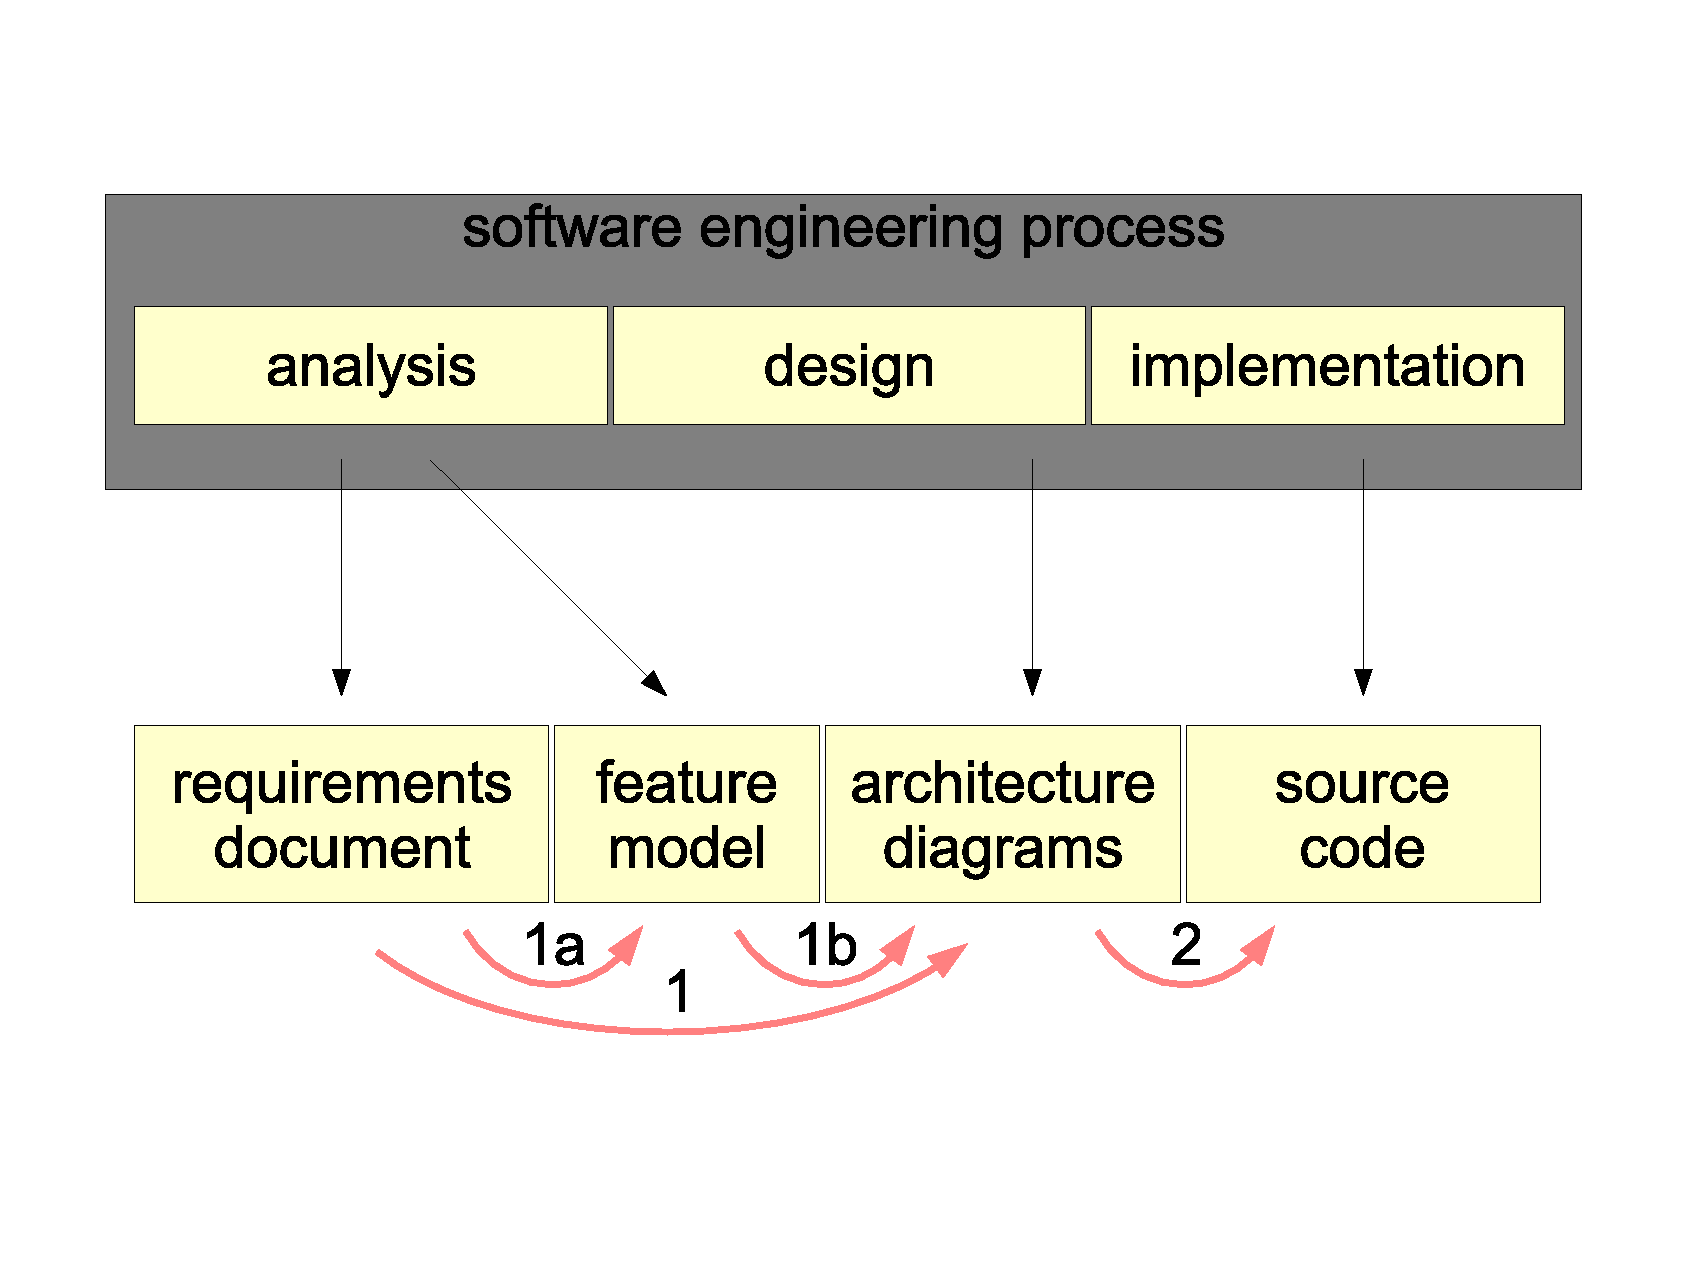
\includegraphics[scale=0.2]{vector/gaps.eps}
        \caption{Abstraction Gaps}
        \label{gaps_figure}
    \end{center}
\end{figure}

Different forms of SEP exist: \emph{Waterfall},\\ \emph{Iterative},
\emph{Extreme Programming} (XP) and \emph{Agile Programming}. But every
project, consciously or not, follows a SEP that sooner-or-later, in one form or
the other, goes through three common phases: \emph{Analysis}, \emph{Design} and
\emph{Implementation}. Each phase creates its own model of what is to be
abstracted in software and it is the differences in exactly these models that
often cause complications.

A previous article \cite{heller2004} mentioned the\\ \emph{Requirements Document},
\emph{Feature Model},\\ \emph{Architecture Diagrams} and \emph{Source Code} as
forms of knowledge abstraction. It also described the following abstraction
gaps (see figure \ref{gaps_figure}) that have to be crossed:

\begin{enumerate}
    \item[1a] Requirements Document -- Feature M.
    \item[1b] Feature Model -- Architecture Diagr.
    \item[2] Architecture Diagrams -- Source Code
\end{enumerate}

By improving the \emph{Traceability} between requirements and the architecture,
feature models (known from system family/ product line engineering) contribute
to minimising gap 1. Together with architecture diagrams, they ease
communication between stakeholders in the SEP, because of their human-readable
form and implementation-independence. But sooner-or-later, also these have to
be transferred into source code, by crossing gap 2.

Bridging or closing these abstraction gaps (sometimes called \emph{Semantic- or
Conceptual Gaps}) is also known as: \textit{achieving higher intentionality}
and remains an unsolved task for software engineering. One aim of the work
described in this article was to contribute to a possible solution, with focus
on \emph{reducing} gap 2, existing between a designed architecture and the
implemented code.

%
% $RCSfile: misleading_tiers.tex,v $
%
% Copyright (c) 2005-2006. Christian Heller. All rights reserved.
%
% Permission is granted to copy, distribute and/or modify this document
% under the terms of the GNU Free Documentation License, Version 1.1 or
% any later version published by the Free Software Foundation; with no
% Invariant Sections, with no Front-Cover Texts and with no Back-Cover
% Texts. A copy of the license is included in the section entitled
% "GNU Free Documentation License".
%
% http://www.cybop.net
% - Cybernetics Oriented Programming -
%
% http://www.resmedicinae.org
% - Information in Medicine -
%
% Version: $Revision: 1.1 $ $Date: 2006-01-03 08:21:45 $ $Author: christian $
% Authors: Christian Heller <christian.heller@tuxtax.de>
%

\subsection{Misleading Tiers}
\label{misleading_tiers_heading}

When distinguishing human- and technical systems, the kinds of
\emph{Communication} are:

\begin{itemize}
    \item[-] Human $\leftrightarrow$ Human
    \item[-] Human $\leftrightarrow$ Computer
    \item[-] Computer $\leftrightarrow$ Computer
\end{itemize}

Each of these relies on different techniques, transport mechanisms, languages
(protocols) and so on. But the general principle after which communication
works, is always the same -- no matter whether technical \emph{Computer}
systems or their biological prototype, the \emph{Human Being}, are considered:
Information is \emph{received}, \emph{stored}, \emph{processed} and \emph{sent}.
Despite these common characteristics, today's \emph{Information Technology}
(IT) environments \cite{hellerkunze} treat communication between a computer
system and a human being differently than that \emph{among} computer systems.

\begin{figure}[ht]
    \begin{center}
        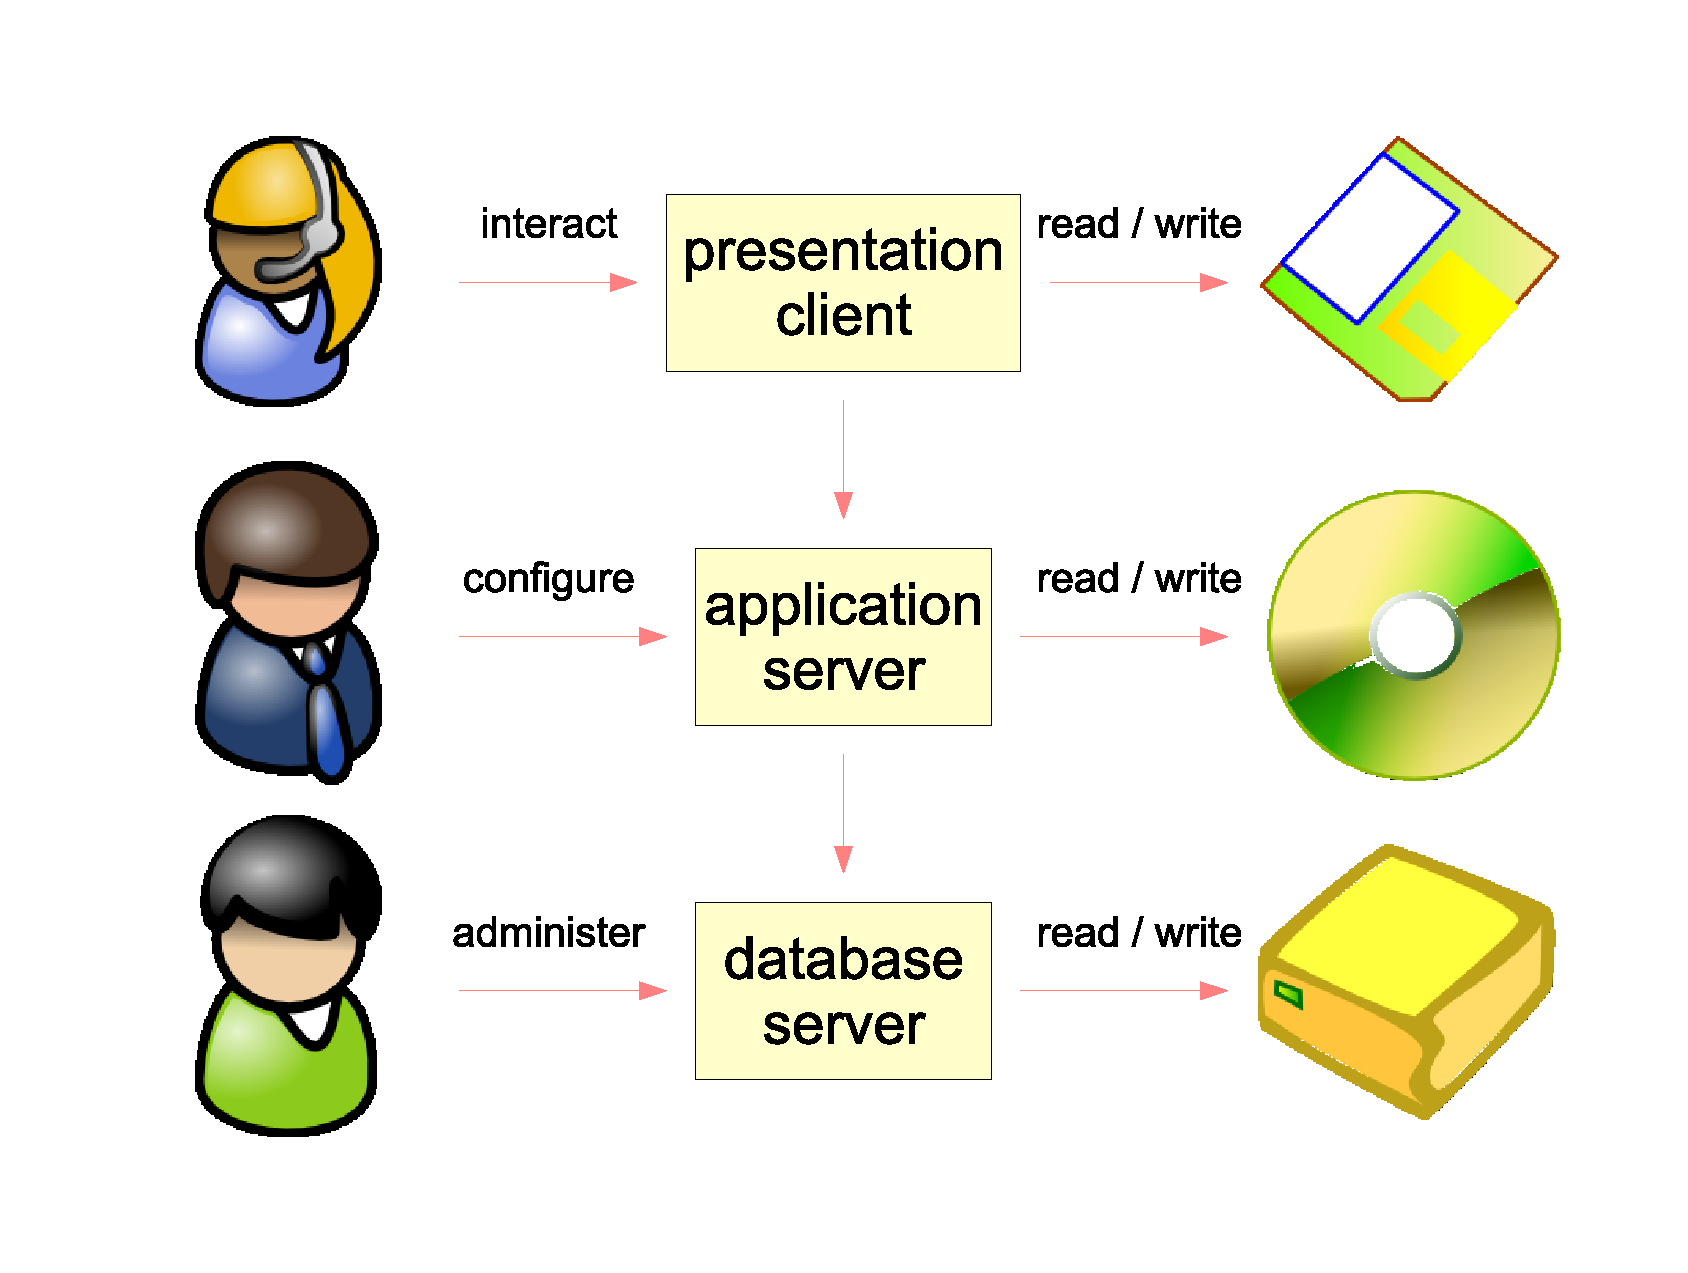
\includegraphics[scale=0.2]{vector/universal.eps}
        \caption{Universal Communication}
        \label{universal_figure}
    \end{center}
\end{figure}

Figure \ref{universal_figure} shows a three-tier environment: tier 1 represents
the \emph{Presentation Layer}; tier 2 stands for the \emph{Application Layer};
tier 3 is the \emph{Database (DB) Layer}. Typical synonyms are, in this order:
\emph{Frontend}, \emph{Business Logic} and \emph{Backend}. The tiers (layers)
serve two needs: connect different locations and share work load (\emph{Scaling}).
However, the split into tiers of that kind raises two illusions:

\begin{enumerate}
    \item \emph{Users only interact with clients}
    \item \emph{Persistent data are stored in DB only}
\end{enumerate}

Many IT architectures, or at least their illustrations, neglect the fact that
in reality \emph{all} systems need a \emph{User Interface} (UI), for at least
being administered by humans, and \emph{almost} all systems, even
\emph{Database Management Systems} (DBMS) themselves, store some of their
persistent data outside a database, for example locally available configuration
information. This is not necessarily a problem for the IT environment as such,
but it is for the internal architecture of software systems. Special solutions
have to deal with frontend (UI framework), business logic (domain patterns) and
backend (data mapping), and often additional mechanisms for local and remote
communication. The serious differences in these design solutions are one root
of well-known problems like multi- directional inter-dependencies between system
parts, that make software difficult to develop and hard to maintain.

One aim of the work described in this article was to investigate possibilities
for a \emph{unification} of communication paradigms, that is high-level design
paradigms rather than low-level protocols, in order to architect software in a
way that allows the computer system it runs on to communicate \emph{universally}.

%
% $RCSfile: modelling_mistakes.tex,v $
%
% Copyright (c) 2005-2006. Christian Heller. All rights reserved.
%
% Permission is granted to copy, distribute and/or modify this document
% under the terms of the GNU Free Documentation License, Version 1.1 or
% any later version published by the Free Software Foundation; with no
% Invariant Sections, with no Front-Cover Texts and with no Back-Cover
% Texts. A copy of the license is included in the section entitled
% "GNU Free Documentation License".
%
% http://www.cybop.net
% - Cybernetics Oriented Programming -
%
% http://www.resmedicinae.org
% - Information in Medicine -
%
% Version: $Revision: 1.1 $ $Date: 2006-01-03 08:21:45 $ $Author: christian $
% Authors: Christian Heller <christian.heller@tuxtax.de>
%

\subsection{Modelling Mistakes}
\label{modelling_mistakes_heading}

Most modern software is not written directly in a machine language but designed
in form of higher-level models instead. These allow to speed up application
development and help avoiding errors. \emph{Object Oriented Programming} (OOP),
for example, uses design concepts like the \emph{Class} owning \emph{Attributes}
and \emph{Methods}. Yet does this kind of modelling create abstractions that
reflect concepts of the real world completely and correctly?

\begin{figure}[ht]
    \begin{center}
        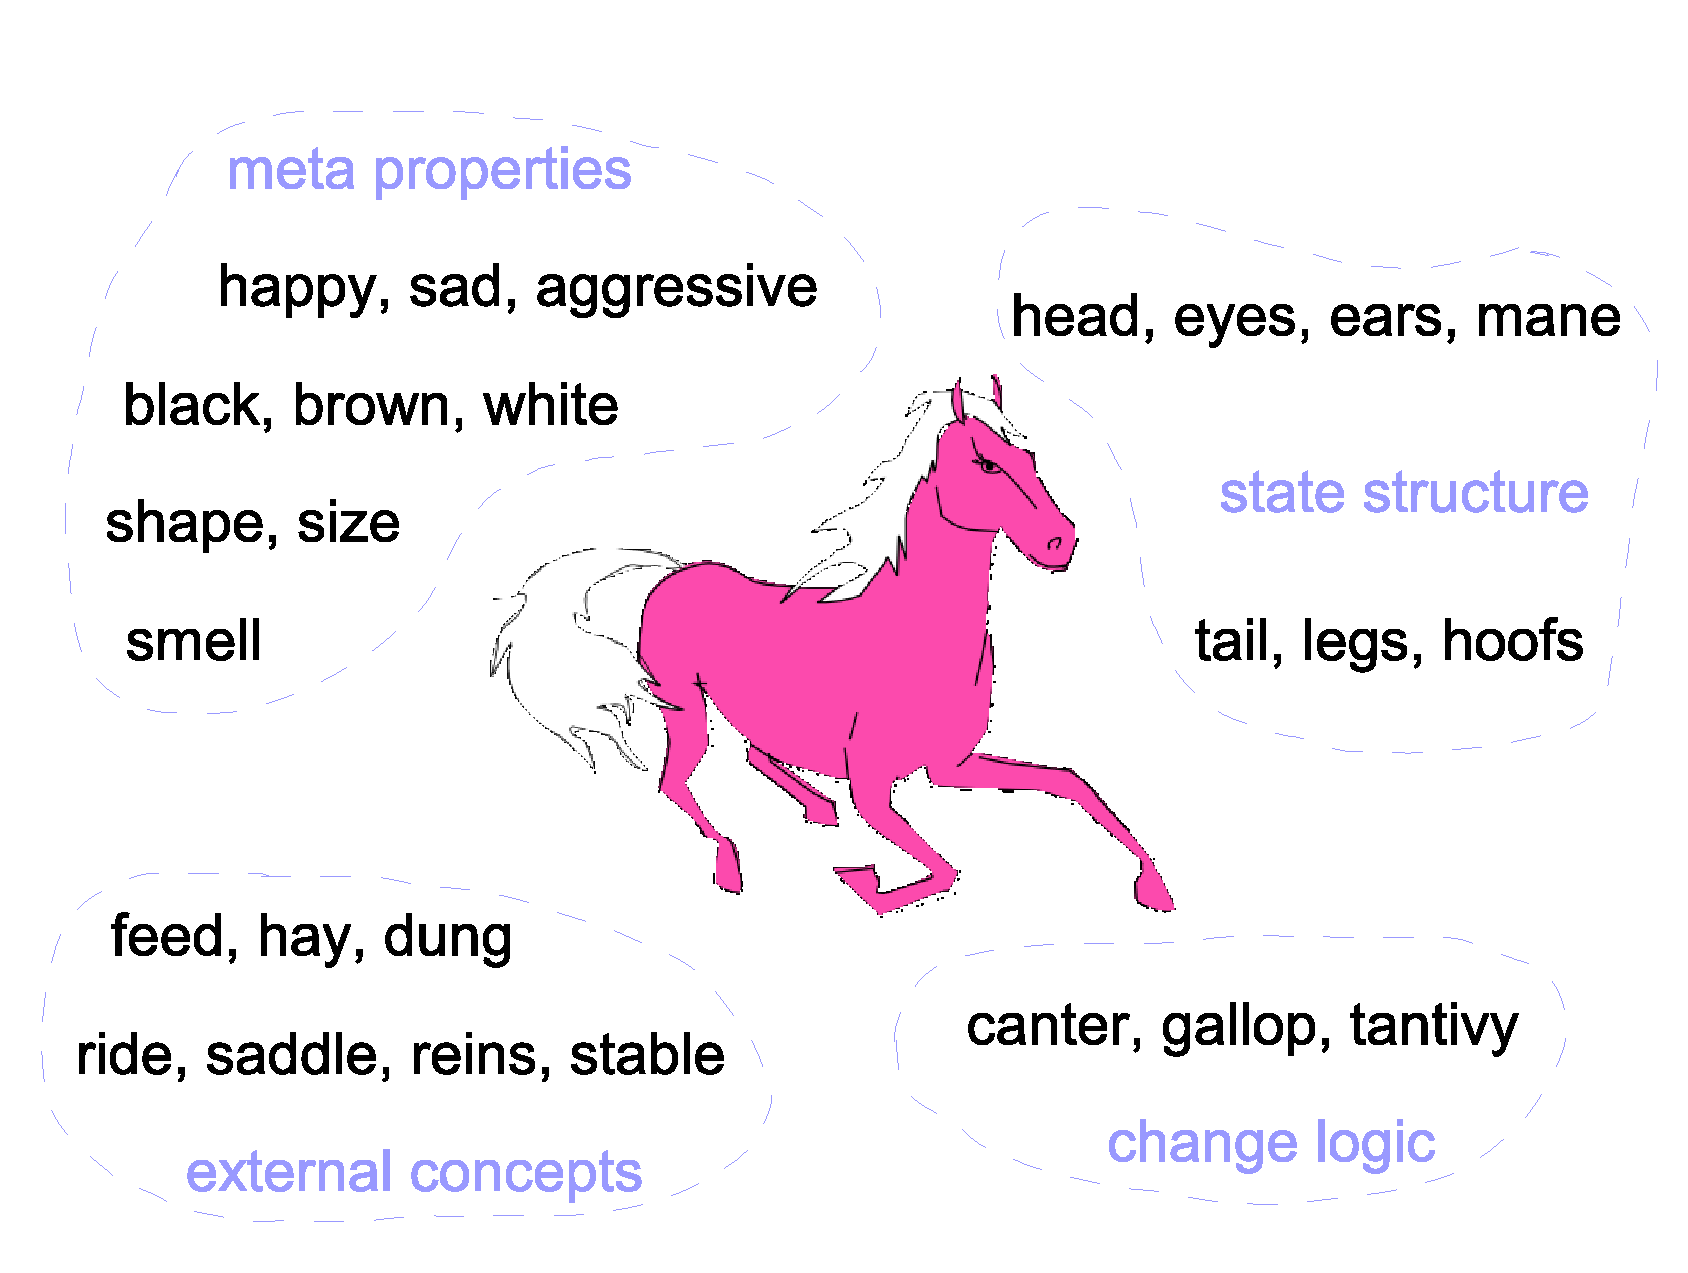
\includegraphics[scale=0.2]{vector/horse.eps}
        \caption{Concept of a Horse}
        \label{horse_figure}
    \end{center}
\end{figure}

The model of a \emph{Horse} shall serve as example to investigate this further.
Figure \ref{horse_figure} shows a number of terms commonly used to describe a
horse. Most importantly, there are structural observations describing the horse
as concept consisting of parts like \emph{Head}, \emph{Legs} or \emph{Hoofs}.
Secondly, there are properties like the horse's \emph{Colour}, \emph{Shape} or
\emph{Size}. Thirdly, there are terms describing a horse's actions like its
\emph{Movement} or \emph{Eating}, that change a horse's position and/ or state.
Finally, there are a number of terms like \emph{Hay} or \emph{Saddle}
associating concepts related to the horse.

One might suggest to model properties like the position, size or colour of a
horse's leg as \emph{Part} of that leg. In fact, this is how classical
programming approaches its solutions. In OOP, one would probably use a class
representing the leg and an attribute standing for the leg's colour. However,
when following the modelling principles of human thinking (see
\cite{heller2004}), this is \emph{not} correct!

It is true that in everyday language, one tends to say \textit{A horse leg
\emph{has a} colour.} Unfortunately, this leads to the wrong assumption that a
leg were made of a colour. But this is not the case. A leg does not
\emph{consist} of a colour in the hierarchical meaning of a whole consisting of
parts. The colour is rather property information \emph{about} the leg. It seems
there is no correct expression in natural (English) language stating the
property of something. The \emph{IS-A} verbalisation is used to express that
the leg belongs to a special category of items, for example: \textit{A leg is a
body element.} The \emph{HAS-A} formulation is used to express that a leg as
whole consists of smaller parts, for example: \textit{A leg has a knee and it
has a hoof.} But which formulation expresses a property? Well, perhaps it would
be best to say: \textit{A leg IS-OF a colour.}

The CYBOP knowledge schema described later in this article distinguishes
structural- from meta information. Actions (like the gallop of a horse) causing
change in the model or its environment are called \emph{Logic} in this work,
since they follow certain rules.


    %
% $RCSfile: pattern.tex,v $
%
% Copyright (c) 2004. Christian Heller. All rights reserved.
%
% No copying, altering, distribution or any other actions concerning this
% document, except after explicit permission by the author!
% At some later point in time, this document is planned to be put under
% the GNU FDL license. For now, _everything_ is _restricted_ by the author.
%
% http://www.cybop.net
% - Cybernetics Oriented Programming -
%
% http://www.resmedicinae.org
% - Information in Medicine -
%
% @author Christian Heller <christian.heller@tuxtax.de>
%

\section{Pattern}
\label{pattern_heading}

%
% $RCSfile: definition.tex,v $
%
% Copyright (c) 2002-2007. Christian Heller. All rights reserved.
%
% Permission is granted to copy, distribute and/or modify this document
% under the terms of the GNU Free Documentation License, Version 1.1 or
% any later version published by the Free Software Foundation; with no
% Invariant Sections, with no Front-Cover Texts and with no Back-Cover
% Texts. A copy of the license is included in the section entitled
% "GNU Free Documentation License".
%
% http://www.cybop.net
% - Cybernetics Oriented Programming -
%
% Version: $Revision: 1.2 $ $Date: 2007-08-01 13:59:00 $ $Author: christian $
% Authors: Christian Heller <christian.heller@tuxtax.de>
%

\chapter{Definition}
\label{definition_heading}
\index{Definition}
\index{Whole-Part Hierarchy}
\index{Meta Data Hierarchy}
\index{Extensible Markup Language}
\index{XML}

This chapter defines the \emph{Syntax}, \emph{Vocabulary} and \emph{Semantics}
of the CYBOL language.

As already mentioned in chapter \ref{introduction_heading}, CYBOL is based upon
\emph{two} kinds of hierarchies. One of them is representing \emph{Whole-Part}
relations (such as a graphical window consisting of a menu bar) and the other
the \emph{Meta Data} which a whole keeps about its parts (such as the size or
colour of the menu bar). More details and the philosophical background are
described in \cite{cybopbook}. The syntax and semantics of CYBOL as new
language must be rich enough to express abstract knowledge models using this
kind of double hierarchy.

%
% $RCSfile: syntax.tex,v $
%
% Copyright (C) 2002-2008. Christian Heller.
%
% Permission is granted to copy, distribute and/or modify this document
% under the terms of the GNU Free Documentation License, Version 1.1 or
% any later version published by the Free Software Foundation; with no
% Invariant Sections, with no Front-Cover Texts and with no Back-Cover
% Texts. A copy of the license is included in the section entitled
% "GNU Free Documentation License".
%
% http://www.cybop.net
% - Cybernetics Oriented Programming -
%
% http://www.resmedicinae.org
% - Information in Medicine -
%
% Version: $Revision: 1.1 $ $Date: 2008-08-19 20:41:09 $ $Author: christian $
% Authors: Christian Heller <christian.heller@tuxtax.de>
%

\subsection{Syntax}
\label{syntax_heading}
\index{CYBOL Syntax}
\index{Syntax of a Language}
\index{Grammar of a Language}
\index{Extensible Markup Language}
\index{XML}
\index{XML Tag}
\index{XML Attribute}
\index{Discrimination}
\index{Composition}

Every language has a special \emph{Syntax}, that is a \emph{Grammar} with rules
for combining terms and symbols \cite{foldoc}. CYBOL could define its own
syntax or use an already existing one, of another language. Because of its
popularity, clear text representation, flexibility, extensibility and ease of
use, \emph{XML} was chosen to deliver the syntax for CYBOL.

To mention just two of the syntactical elements of XML, \emph{Tag} and
\emph{Attribute} are considered shortly here. Tags are special, arbitrary
keywords that have to be defined by the system working with an XML document.
Attributes keep additional information about the contents enclosed by two tags.
Two examples:

\begin{scriptsize}
    \begin{verbatim}
    <tag attribute="value">
        contents
    </tag>
    \end{verbatim}
\end{scriptsize}

\begin{scriptsize}
    \begin{verbatim}
    <tag attribute1="value" attribute2="contents"/>
    \end{verbatim}
\end{scriptsize}

An XML document carries a name and can such represent a \emph{Discrete Item},
as suggested by the principles of human thinking (section
\ref{human_thinking_heading}). Being a \emph{Compound}, it consists of parts --
and, it can link to other documents treated as its parts. That way, a whole
hierarchy can be formed. Tag attributes can keep additional information about
the linked parts. Most importantly, XML documents have a hierarchical structure
based on tags, which may be used to store meta information about a part.

Considering these properties of XML, it seems predestinated for formally
representing abstract models using the CYBOP concepts. CYBOL, finally, is XML
\emph{plus} a defined set of tags, attributes and values, used to structure and
link documents meaningfully.

%
% $RCSfile: vocabulary.tex,v $
%
% Copyright (c) 2001-2004. Christian Heller. All rights reserved.
%
% No copying, altering, distribution or any other actions concerning this
% document, except after explicit permission by the author!
% At some later point in time, this document is planned to be put under
% the GNU FDL license. For now, _everything_ is _restricted_ by the author.
%
% http://www.cybop.net
% - Cybernetics Oriented Programming -
%
% http://www.resmedicinae.org
% - Information in Medicine -
%
% @author Christian Heller <christian.heller@tuxtax.de>
%

\subsection{Vocabulary}
\label{vocabulary_heading}

XML allows to define and exchange the whole vocabulary of a language. It offers
two ways in which a list of legal elements can be defined: The traditional
\emph{Document Type Definition} (DTD) and the more modern \emph{XML Schema
Definition} (XSD). Besides the vocabulary, DTD and XSD define the structure of
an XML document and allow to typify, constrain and validate items. The CYBOL DTD
and XSD can be found at \cite{cybop}.

%
% $RCSfile: semantics.tex,v $
%
% Copyright (c) 2002-2007. Christian Heller. All rights reserved.
%
% Permission is granted to copy, distribute and/or modify this document
% under the terms of the GNU Free Documentation License, Version 1.1 or
% any later version published by the Free Software Foundation; with no
% Invariant Sections, with no Front-Cover Texts and with no Back-Cover
% Texts. A copy of the license is included in the section entitled
% "GNU Free Documentation License".
%
% http://www.cybop.net
% - Cybernetics Oriented Programming -
%
% Version: $Revision: 1.1 $ $Date: 2007-08-01 13:59:00 $ $Author: christian $
% Authors: Christian Heller <christian.heller@tuxtax.de>
%

\section{Semantics}
\label{semantics_heading}
\index{Semantics}
\index{State Knowledge Modelling}
\index{Logic Knowledge Modelling}
\index{Extensible Markup Language}
\index{XML}
\index{XML Tag}
\index{XML Attribute}

The meaning expressed by terms and sentences is their \emph{Semantics}
\cite{duden}.

CYBOL files can be used to model \emph{State Knowledge} (like a graphical
window or a person's address) and \emph{Logic Knowledge} (like an operation or
algorithm or workflow) \cite{cybopbook}. In both cases, the \emph{same} syntax
(document structure) with \emph{identical} vocabulary (XML tags and -attributes)
is applied. It is the attribute \emph{Values} that make a difference in meaning.

The double hierarchy mentioned before is realised in CYBOL knowledge templates
by using XML \emph{Attributes} for representing the whole-part hierarchy, and
XML \emph{Tags} for representing the additional meta data that a whole model
keeps about its part models.

\input{attributes}
\input{tags}
\input{tag_attribute_swapping}


%
% $RCSfile: classification.tex,v $
%
% Copyright (C) 2002-2008. Christian Heller.
%
% Permission is granted to copy, distribute and/or modify this document
% under the terms of the GNU Free Documentation License, Version 1.1 or
% any later version published by the Free Software Foundation; with no
% Invariant Sections, with no Front-Cover Texts and with no Back-Cover
% Texts. A copy of the license is included in the section entitled
% "GNU Free Documentation License".
%
% http://www.cybop.net
% - Cybernetics Oriented Programming -
%
% http://www.resmedicinae.org
% - Information in Medicine -
%
% Version: $Revision: 1.1 $ $Date: 2008-08-19 20:41:05 $ $Author: christian $
% Authors: Christian Heller <christian.heller@tuxtax.de>
%

\subsubsection{Classification}
\label{classification_heading}
\index{Classification}
\index{Class}
\index{Attribute}
\index{Method}
\index{Structured Data Type}
\index{Struct}
\index{Record}
\index{Structured and Procedural Programming}
\index{SPP}
\index{Java}
\index{Global Variable}
\index{Instance}
\index{Object}
\index{Instantiation}
\index{Abstract Class}
\index{Interface}
\index{Inner Class}
\index{Bundling of Attributes and Methods}

The main idea of object oriented programming is to structure program code into
\emph{Classes} owning \emph{Attributes} and \emph{Methods} (figure
\ref{classification_figure}). They are comparable to the structured data types
(\emph{struct}, \emph{record}) of \emph{Structured and Procedural Programming}
(SPP) (section \ref{structured_and_procedural_programming_heading}) that can
own fields representing properties, but not behaviour. A class definition in
\emph{Java} source code looks like this:

\begin{scriptsize}
    \begin{verbatim}
    public class Example {
        private Type attribute;
        public void method(Type parameter) {
        }
    }
    \end{verbatim}
\end{scriptsize}

\begin{figure}[ht]
    \begin{center}
        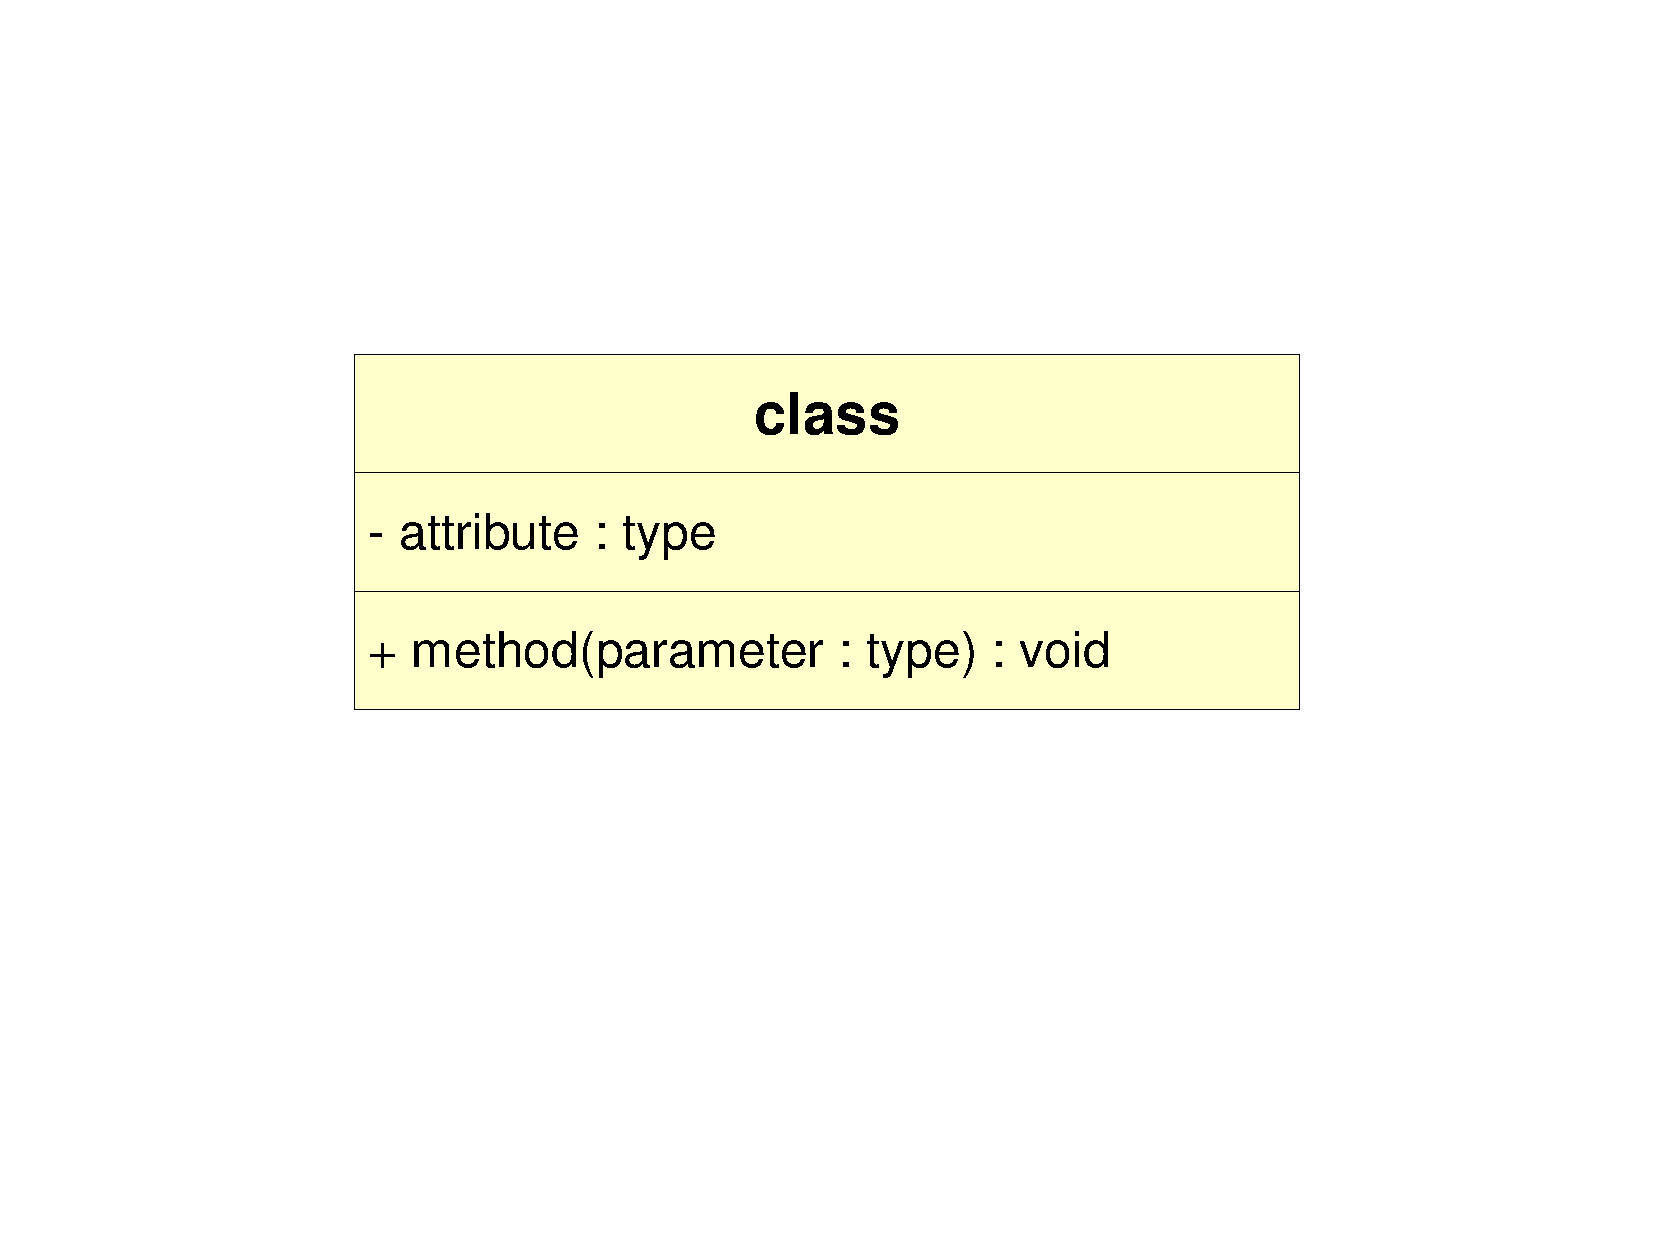
\includegraphics[scale=0.3,angle=-90]{graphic/classification.pdf}
        \caption{Classification as UML Diagram}
        \label{classification_figure}
    \end{center}
\end{figure}

While procedures and many variables in SPP are global, that is only exist once,
classes are treated as types of which many \emph{Instances} (also called
\emph{Objects}) can be created, including attributes and methods. In OOP, such
memory allocation is called \emph{Instantiation}.

Two related data types are \emph{Abstract Class} and \emph{Interface}. An
abstract class can hold attributes and (partly abstract) methods. Just like
interfaces, abstract classes cannot be instantiated. An interface is yet more
restricted in that it can only have constants but not attributes and only
declarations but not actual implementations of methods. Interfaces are commonly
used to \cite{steppan}:

\begin{itemize}
    \item[-] Realise multiple inheritance (section \ref{inheritance_heading})
    \item[-] Encapsulate components (section \ref{interface_and_implementation_heading})
    \item[-] Pool common methods (section \ref{separation_of_concerns_heading})
\end{itemize}

Specialities like \emph{Inner Classes} \cite{java} with limited scope of
validity are of minor importance to the argumentation of this document and not
further explained here.

The \emph{Bundling} of attributes and methods (state and logic) causes more
system interdependencies and complications than were predictable. It is a big
disadvantage that affects all modern object-oriented systems. \cite{heller2004}
Certainly, the bundling stems from best intentions to receive cleaner code by
keeping not only attributes but also methods in a common module, such avoiding
\emph{wild} and \emph{global} procedures. But now, modules not only have to
refer to other modules for accessing their state data; the same is needed for
accessing their logic in form of method calls.

With OOP, the number of cross-relations between modules, and inter-dependencies
between system layers may rise dramatically. In reality, state- and logic
properties are two \emph{different} things that have to be kept in different
places! Both can have a similar, hierarchical structure but each is a concept on
its own, as chapter \ref{state_and_logic_heading} will show.

%
% $RCSfile: examples.tex,v $
%
% Copyright (c) 2002-2007. Christian Heller. All rights reserved.
%
% Permission is granted to copy, distribute and/or modify this document
% under the terms of the GNU Free Documentation License, Version 1.1 or
% any later version published by the Free Software Foundation; with no
% Invariant Sections, with no Front-Cover Texts and with no Back-Cover
% Texts. A copy of the license is included in the section entitled
% "GNU Free Documentation License".
%
% http://www.cybop.net
% - Cybernetics Oriented Programming -
%
% Version: $Revision: 1.1 $ $Date: 2007-08-01 13:59:00 $ $Author: christian $
% Authors: Christian Heller <christian.heller@tuxtax.de>
%

\chapter{Examples}
\label{examples_heading}
\index{Examples}

The following examples demonstrate how CYBOL's constructs may be used in
practice. Also, attention is payed to how control structures of classical
programming languages may be implemented in CYBOL. Furthermore, this section
discusses how inheritance, containers and software patterns were considered in
the design of CYBOL.

%
% $RCSfile: state_examples.tex,v $
%
% Copyright (C) 2002-2008. Christian Heller.
%
% Permission is granted to copy, distribute and/or modify this document
% under the terms of the GNU Free Documentation License, Version 1.1 or
% any later version published by the Free Software Foundation; with no
% Invariant Sections, with no Front-Cover Texts and with no Back-Cover
% Texts. A copy of the license is included in the section entitled
% "GNU Free Documentation License".
%
% http://www.cybop.net
% - Cybernetics Oriented Programming -
%
% http://www.resmedicinae.org
% - Information in Medicine -
%
% Version: $Revision: 1.1 $ $Date: 2008-08-19 20:41:09 $ $Author: christian $
% Authors: Christian Heller <christian.heller@tuxtax.de>
%

\subsection{State Examples}
\label{state_examples_heading}
\index{CYBOL State Example Constructs}

The creation of composed state models is quite straightforward and clear, as
the following CYBOL knowledge templates show.

\input{model_part_relation}
\input{meta_properties}
\input{external_resources}
\input{serialised_model}
\input{meta_constraints}

%
% $RCSfile: logic_examples.tex,v $
%
% Copyright (C) 2002-2008. Christian Heller.
%
% Permission is granted to copy, distribute and/or modify this document
% under the terms of the GNU Free Documentation License, Version 1.1 or
% any later version published by the Free Software Foundation; with no
% Invariant Sections, with no Front-Cover Texts and with no Back-Cover
% Texts. A copy of the license is included in the section entitled
% "GNU Free Documentation License".
%
% http://www.cybop.net
% - Cybernetics Oriented Programming -
%
% http://www.resmedicinae.org
% - Information in Medicine -
%
% Version: $Revision: 1.1 $ $Date: 2008-08-19 20:41:07 $ $Author: christian $
% Authors: Christian Heller <christian.heller@tuxtax.de>
%

\subsection{Logic Examples}
\label{logic_examples_heading}
\index{CYBOL Logic Example Constructs}

The CYBOL implementation of logic models (chapter \ref{state_and_logic_heading})
needs more detailed explanation, in particular the use of special control
structures as known from \emph{Structured and Procedural Programming} (SPP)
(section \ref{structured_and_procedural_programming_heading}).

\input{operation_call}
\input{algorithm_division}
\input{simple_assignment}
\input{loop_as_operation}
\input{conditional_execution}

%
% $RCSfile: special_examples.tex,v $
%
% Copyright (C) 2002-2008. Christian Heller.
%
% Permission is granted to copy, distribute and/or modify this document
% under the terms of the GNU Free Documentation License, Version 1.1 or
% any later version published by the Free Software Foundation; with no
% Invariant Sections, with no Front-Cover Texts and with no Back-Cover
% Texts. A copy of the license is included in the section entitled
% "GNU Free Documentation License".
%
% http://www.cybop.net
% - Cybernetics Oriented Programming -
%
% http://www.resmedicinae.org
% - Information in Medicine -
%
% Version: $Revision: 1.1 $ $Date: 2008-08-19 20:41:09 $ $Author: christian $
% Authors: Christian Heller <christian.heller@tuxtax.de>
%

\subsection{Special Examples}
\label{special_examples_heading}
\index{CYBOL Special Example Constructs}

\emph{XML} is used for representing data of very different domains, and a whole
plethora of XML dialects exists. Two of them are mentioned following. The main
purpose of the next examples, however, is to show how CYBOL can replace these.

\input{synchronous_execution}
\input{presentation_and_content}
\input{hello_world}
\input{any_system}

%
% $RCSfile: inheritance_as_property.tex,v $
%
% Copyright (c) 2002-2007. Christian Heller. All rights reserved.
%
% Permission is granted to copy, distribute and/or modify this document
% under the terms of the GNU Free Documentation License, Version 1.1 or
% any later version published by the Free Software Foundation; with no
% Invariant Sections, with no Front-Cover Texts and with no Back-Cover
% Texts. A copy of the license is included in the section entitled
% "GNU Free Documentation License".
%
% http://www.cybop.net
% - Cybernetics Oriented Programming -
%
% Version: $Revision: 1.1 $ $Date: 2007-08-01 13:59:00 $ $Author: christian $
% Authors: Christian Heller <christian.heller@tuxtax.de>
%

\section{Inheritance as Property}
\label{inheritance_as_property_heading}
\index{Inheritance as CYBOL Property}

One fundamental concept of \emph{Object Oriented Programming} (OOP) is
\emph{Inheritance}. In principle, there is no problem with implementing
inheritance in CYBOL. If done, however, it would differ from traditional class
architectures as known from OOP. Classical OOP systems resolve inheritance
relationships at runtime; CYBOP systems, on the other hand, would resolve them
just once when creating a knowledge model (instance) from a knowledge template.
After instantiation, all inheritance relationships are lost since instances are
stored as purely hierarchical \emph{whole}-\emph{part} models in memory,
without any links to \emph{super} models.

The following knowledge template shows how inheritance could be realised in
CYBOL. Contrary to OOP classes which hold a link to their corresponding
\emph{super} class as \emph{intrinsic} property, a CYBOL knowledge template
does not know itself from which \emph{super} template to inherit from. That
information is stored as \emph{extrinsic} property outside the template
instead, in other words in the \emph{whole} template to which the inheriting
template belongs.

\begin{scriptsize}
    \begin{verbatim}
<model>
    <part name="ok_button" channel="file" abstraction="cybol" model="gui/ok_button.cybol">
        <property name="super" channel="file" abstraction="cybol" model="button.cybol"/>
        <property name="size" channel="inline" abstraction="integer" model="90,30,1"/>
        <property name="colour" channel="inline" abstraction="rgb" model="127,127,127"/>
    </part>
</model>
    \end{verbatim}
\end{scriptsize}

One of the properties in the example template above carries the name
\emph{super}. Its model references another template which is treated as super
template of the corresponding \emph{part} the property belongs to. With slight
modifications on the property name \emph{super}, which has to be unique among
all properties of a part, it would even be possible to implement
\emph{Multiple Inheritance}. Dependency complications are not to be expected
because all inheritance relationships are forgotten in runtime models.

Although the described inheritance mechanism was tested successfully in an
older prototype application, it has not been implemented in CYBOL. None of the
created example applications showed a need for it, nor did any of them promise
more effective programming. The reuse of CYBOL templates is realised through
composition only, that is fine-granular templates make up more coarse-grained
ones. This counts for both, state- as well as logic models, since they are not
bundled like in OOP. And polymorphism as effect does not have to be considered.

%
% $RCSfile$
%
% Copyright (c) 2005-2006. Christian Heller. All rights reserved.
%
% Permission is granted to copy, distribute and/or modify this document
% under the terms of the GNU Free Documentation License, Version 1.1 or
% any later version published by the Free Software Foundation; with no
% Invariant Sections, with no Front-Cover Texts and with no Back-Cover
% Texts. A copy of the license is included in the section entitled
% "GNU Free Documentation License".
%
% http://www.cybop.net
% - Cybernetics Oriented Programming -
%
% http://www.resmedicinae.org
% - Information in Medicine -
%
% Version: $Revision$ $Date$ $Author$
% Authors: Christian Heller <christian.heller@tuxtax.de>
%

\subsubsection{Container Mapping}
\label{container_mapping_heading}

State-of-the-art programming languages offer a number of different container
types, partly based on each other through inheritance. Sections
\ref{motivation_heading} and \ref{container_unification_heading} of this work
mentioned \emph{Container Inheritance} as one reason for falsified program
results.

\begin{table}[ht]
    \begin{center}
        \begin{tabular}{| p{15mm} | p{35mm} |}
            \hline
            \textbf{Container} & \textbf{Knowledge Template}\\
            \hline
            Tree & Hierarchical \emph{whole}-\emph{part} structure\\
            \hline
            Table & Like a Tree, as hierarchy consisting of rows which consist of columns\\
            \hline
            Map & Parts have a \emph{name} (key) and a \emph{model} (value)\\
            \hline
            List & Parts may have a \emph{position} property\\
            \hline
            Vector & A \emph{model} attribute may hold comma-separated values;
                a template holds a number of parts (dynamically changeable)\\
            \hline
            Array & Like a Vector; characters are interpreted as \emph{string}\\
            \hline
        \end{tabular}
        \caption{Containers in CYBOL}
        \label{mapping_table}
    \end{center}
\end{table}

Section \ref{knowledge_schema_heading} introduced a \emph{Knowledge Schema}
which represents each item as \emph{Hierarchy} by default, the result being
that different types of containers are not needed any longer. But how are the
different kinds of container behaviour implemented in CYBOL? Table
\ref{mapping_table} gives an answer.

%
% $RCSfile: hidden_patterns.tex,v $
%
% Copyright (C) 2002-2008. Christian Heller.
%
% Permission is granted to copy, distribute and/or modify this document
% under the terms of the GNU Free Documentation License, Version 1.1 or
% any later version published by the Free Software Foundation; with no
% Invariant Sections, with no Front-Cover Texts and with no Back-Cover
% Texts. A copy of the license is included in the section entitled
% "GNU Free Documentation License".
%
% http://www.cybop.net
% - Cybernetics Oriented Programming -
%
% http://www.resmedicinae.org
% - Information in Medicine -
%
% Version: $Revision: 1.1 $ $Date: 2008-08-19 20:41:07 $ $Author: christian $
% Authors: Christian Heller <christian.heller@tuxtax.de>
%

\subsection{Hidden Patterns}
\label{hidden_patterns_heading}
\index{Patterns in CYBOL}
\index{Hidden Patterns in CYBOL}

There are a number of software patterns (section \ref{pattern_heading}) that
may not be obvious (hidden) at first sight, but have been considered in the
design of the CYBOL language.

Most obviously, CYBOL knowledge templates follow the \emph{Composite} pattern,
in a simplified form. All templates represent a compound consisting of part
templates, which leads to a tree-like structure. But this also means that related
patterns (see section \ref{pattern_systematics_heading}) like \emph{Whole-Part}
and \emph{Wrapper} are representable by CYBOL knowledge templates. A template
as whole wraps its parts.

Knowledge templates with similar granularity can be collected in one directory,
in other words one common ontological level. Templates with smaller granularity,
that is those that the more coarse-grained templates consist of, can be placed
in another common layer and so forth. What comes out of it is a system of levels
-- one variant of the \emph{Layers} pattern.



    %
% $RCSfile: problems.tex,v $
%
% Copyright (c) 2004. Christian Heller. All rights reserved.
%
% No copying, altering, distribution or any other actions concerning this
% document, except after explicit permission by the author!
% At some later point in time, this document is planned to be put under
% the GNU FDL license. For now, _everything_ is _restricted_ by the author.
%
% http://www.cybop.net
% - Cybernetics Oriented Programming -
%
% http://www.resmedicinae.org
% - Information in Medicine -
%
% @author Christian Heller <christian.heller@tuxtax.de>
%

\section{Problems}
\label{problems_heading}

This section does not describe further patterns. Instead, it wants to come back
to reflective- and other mechanisms as described in section \ref{pattern_heading}
before, and elaborate their negative effects a bit more. Although the first of
the following three reviews concentrates on the example of \emph{Java}, many
points surely count for other \emph{Object Oriented Programming} (OOP) languages
as well.

%
% $RCSfile: broken_type_system.tex,v $
%
% Copyright (c) 2004. Christian Heller. All rights reserved.
%
% No copying, altering, distribution or any other actions concerning this
% document, except after explicit permission by the author!
% At some later point in time, this document is planned to be put under
% the GNU FDL license. For now, _everything_ is _restricted_ by the author.
%
% http://www.cybop.net
% - Cybernetics Oriented Programming -
%
% http://www.resmedicinae.org
% - Information in Medicine -
%
% @author Christian Heller <christian.heller@tuxtax.de>
%

\subsection{Broken Type System}
\label{broken_type_system_heading}

Languages like \emph{Smalltalk} or the \emph{Common Lisp Object System} (CLOS)
offer reflective mechanisms \cite{buschmann}. The \emph{C++ Standard Library},
also known as \emph{libstdc++} \cite{libstdcpp}, has a \emph{type\_info} class
providing meta information that \emph{C++} innately does not have.

In the \emph{Java} framework \cite{java}, finally, the basic \emph{java.lang.*}
package contains the top-most super class \emph{java.lang.Object}. All other
classes in the framework inherit from it. Additionally, the package contains a
class \emph{java.lang.Class} which, among others, keeps reflective (meta) type
information about a \emph{Java} class':

\begin{itemize}
    \item[-] Package
    \item[-] Name
    \item[-] Superior Class
    \item[-] Interfaces
    \item[-] Fields
    \item[-] Methods
    \item[-] Constructors
    \item[-] Modifiers
    \item[-] Member Classes
\end{itemize}

\begin{figure}[ht]
    \begin{center}
        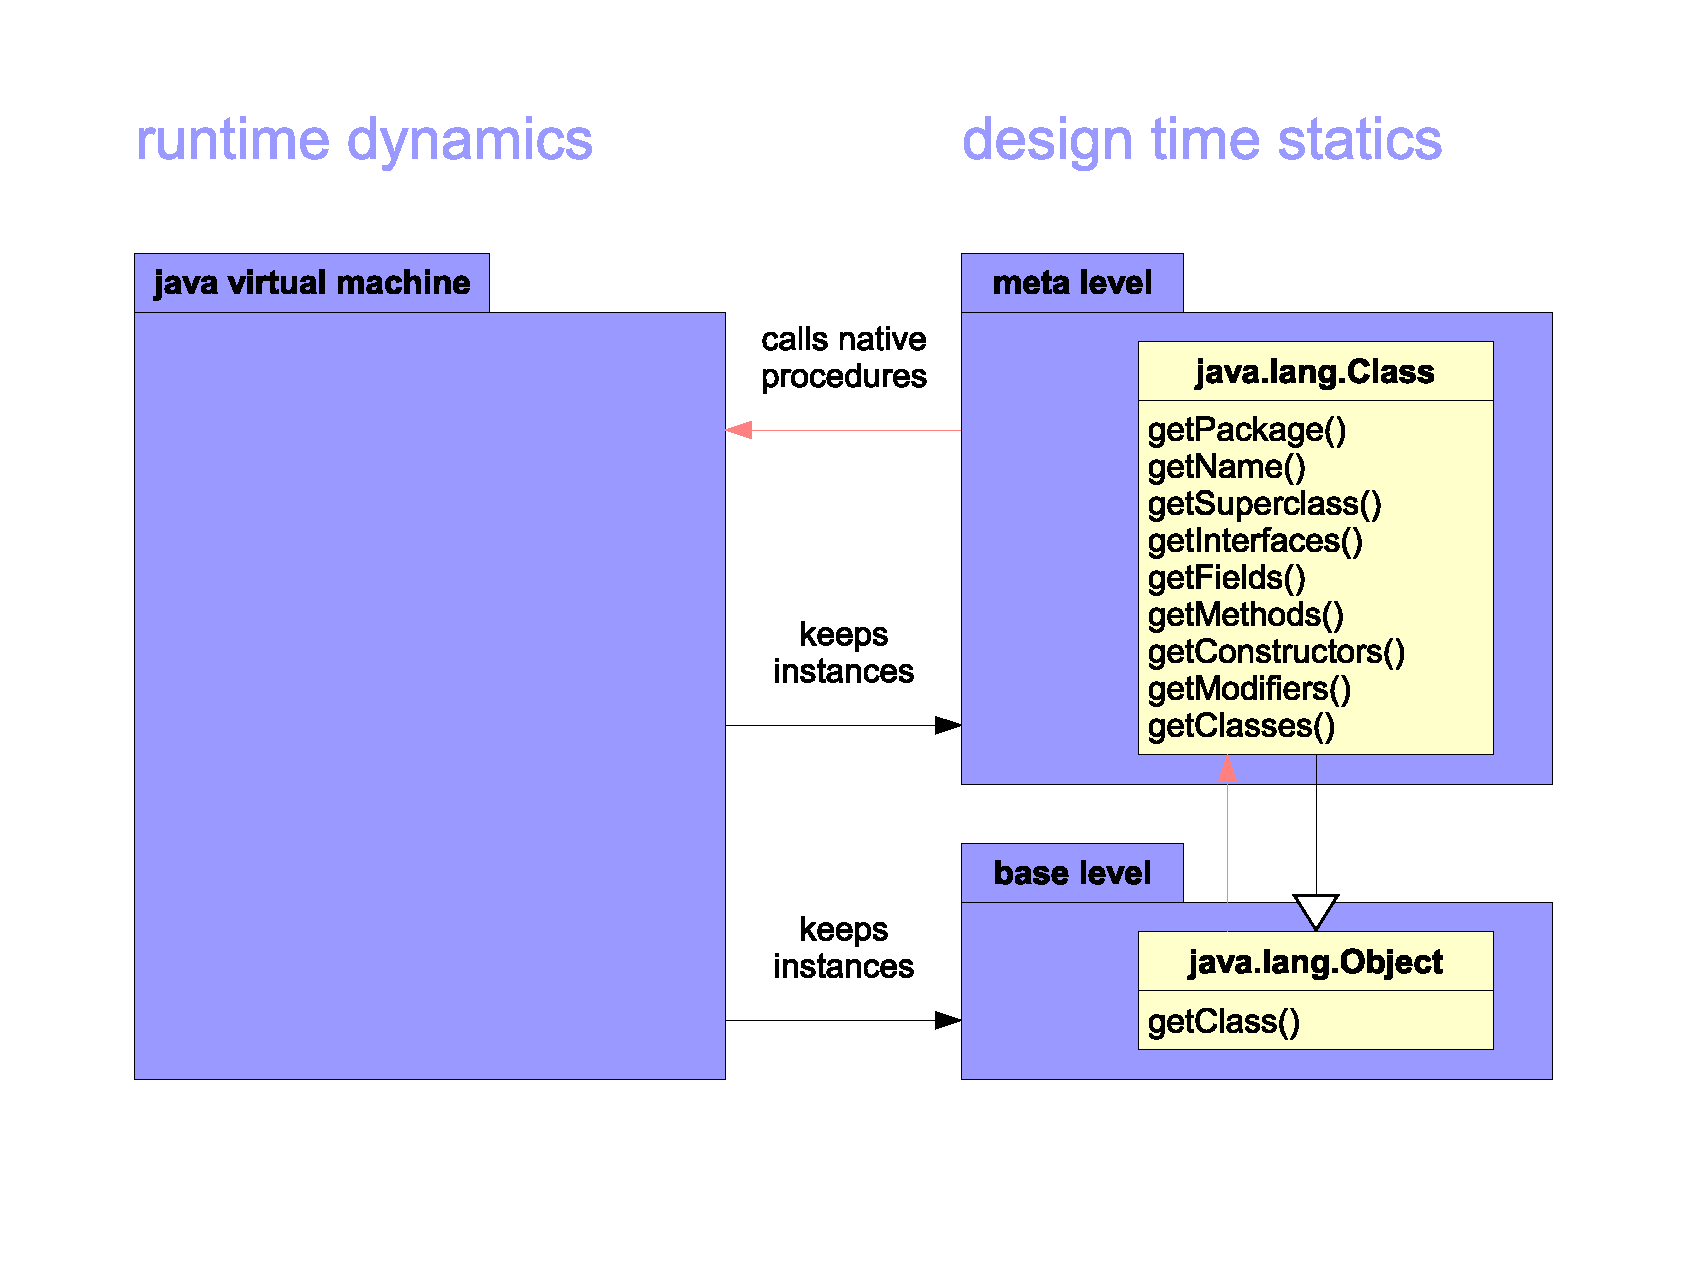
\includegraphics[scale=0.3]{vector/typesystem.eps}
        \caption{Java Type System}
        \label{typesystem_figure}
    \end{center}
\end{figure}

Via the \emph{getClass()} method which they inherit from \emph{java. lang.Object}
(figure \ref{typesystem_figure}), all Java classes have access to that reflective
information in their meta class. The meta class \emph{java.lang.Class} itself
uses so-called \emph{native} methods to access the information in the
\emph{Java Virtual Machine} (JVM).

The JVM operates on a level underneath the actual application, close to the
\emph{Operating System} (OS). It interprets the Java application source code and
resolves all object-oriented- into procedural structures, and finally low-level
system instructions. All runtime objects, that is class instances, are hold in
dynamic structures internal to the JVM. That is why \emph{native} methods need
to be used to access and change the runtime structure or behaviour of objects.

One problem that becomes obvious when inspecting figure \ref{typesystem_figure}
is the existence of a \emph{Bidirectional Dependency}, also called
\emph{Circular Reference}. The two sub dependencies causing it are:

\begin{enumerate}
    \item \emph{Inheritance} of \emph{java.lang.Class} from \emph{java.lang.Object}
        which is due to the rule that all Java classes need to inherit from the
        top-most framework class
    \item \emph{Association} from \emph{java.lang.Object} to \emph{java.lang.Class}
        which enables every object to access its meta class using the
        \emph{getClass()} method
\end{enumerate}

The avoidance of circular references is one of the most basic principles of
computer programming (section \ref{bidirectional_dependency_heading}). The
disadvantage of bidirectional dependencies between meta- and basic level is
also mentioned by Buschmann \cite{buschmann}. If meta classes in the kind of
\emph{java.lang.Class} define the structure and behaviour of all basic classes
inheriting from \emph{java.lang. Object}, then those meta classes in turn should
\emph{not} themselves inherit from \emph{java.lang.Object}.

Another problem is the mixed and redundant storage of meta information which
Jonathon Tidswell \cite{josgeneral} even calls a \emph{Broken Type System}. He
writes: \textit{A careful examination of the classes in the standard runtime will
show that they are not strictly instances of java.lang.Class (hint: statics).}
Gilbert Carl Herschberger II \cite{josgeneral} calls the separation of
reflection and wrappers an \emph{Inconsistent Design}. Java classes are based
on many different kinds of type information:

\begin{itemize}
    \item[-] Structure applied by the JVM through the usage of the \emph{class} keyword
    \item[-] Meta information supplied by the \emph{java.lang.Class} class
    \item[-] Reflective information provided by \emph{java.lang.reflect.*}
    \item[-] Wrapper classes for primitive types in \emph{java.lang.*}
    \item[-] Dynamically created array classes, without having an array class file
\end{itemize}

The fact that the \emph{java.lang.Class} class which is to provide meta
information \emph{about} classes is a \emph{Class} itself is an antagonism. It
is true that that meta class is made \emph{final} to avoid its extension by
inheriting subclasses. But correctly, it should not be a class at all.

Yet how can this paradoxon be resolved? Obviously, one of the two dependencies
between \emph{java.lang.Object} and \emph{java.lang.Class} needs to be cut. But
then either the \emph{java.lang. Object} class would not be able to access its meta
information anymore or the \emph{java.lang.Class} class would not be available as
runtime object to other polymorphic data structures. One solution could be to
merge both classes, so that each object, by default, has the necessary methods
to access its meta information. But as it turns out, this would not be a real
solution, just a \emph{Shift} of the problem to another level. As mentioned above,
the JVM keeps all instances (objects) in internal, dynamic structures. If objects
were allowed to access these internal structures via native methods (procedures),
a similar kind of bidirectional dependency, between the JVM and its stored objects,
would occur.

One finally has to ask whether the usage and manipulation of meta information is
really necessary at all! If objects did not have a \emph{static} structure
consisting of certain attributes and methods, as defined by the software
developer at design time, but instead based on a uniform, \emph{dynamically}
changeable structure -- the need to use reflective mechanisms might disappear.
More research has to be done on this topic.

There are other Java-related points to be criticised. Although it is worth
noting they exist, these are \emph{not} explained in detail here, since this
document wants to focus on general concepts. Gilbert Carl Herschberger II
\cite{josgeneral} mentions the problematic issue of \emph{Pre-Conditions},
leading to corresponding \emph{Assumptions}. After him, such work-arounds were
necessary to break circular references in Java:

\begin{itemize}
    \item[-] Each JVM must pre-define an \emph{Internal Meta Class}, implemented
        in machine code and \emph{not} available as Java bytecode in a class file.
        The \emph{java.lang.Class} as base meta class for all Java classes depends
        on that internal meta class and assumes its existance.
    \item[-] A JVM pre-defines one \emph{Primordial Class Loader}, implemented in
        machine code and resolved at compile-time. Since additional class loaders
        need to know their meta class when being created, they have to assume the
        primordial class loader exists so that, using it, their meta class can be
        created first.
\end{itemize}

Jonathon Tidswell \cite{josgeneral} is of the opinion that there are a number of
security issues related to the design of Java, for example:

\begin{itemize}
    \item[-] Global names not local references are used for security
    \item[-] Wrappers and names are used for reflection
\end{itemize}

Even though most of the issues raised in this section are rather Java-specific,
many of them apply to other programming languages as well. \emph{Smalltalk}
\cite{smalltalk} and \emph{CLU} \cite{clu}, for example, make primitive types
look like classes and do not need special \emph{Wrapper} classes like Java. But
when digging deep enough, one will find that this is \emph{Syntactic Sugar}, as
Peter J. Landin used to call additions to the syntax of a computer language
that do not affect its expressiveness but make it \emph{sweeter} for humans to
use \cite{wikipedia}.

%
% $RCSfile: bidirectional_dependency.tex,v $
%
% Copyright (c) 2004. Christian Heller. All rights reserved.
%
% No copying, altering, distribution or any other actions concerning this
% document, except after explicit permission by the author!
% At some later point in time, this document is planned to be put under
% the GNU FDL license. For now, _everything_ is _restricted_ by the author.
%
% http://www.cybop.net
% - Cybernetics Oriented Programming -
%
% http://www.resmedicinae.org
% - Information in Medicine -
%
% @author Christian Heller <christian.heller@tuxtax.de>
%

\subsection{Bidirectional Dependency}
\label{bidirectional_dependency_heading}

\emph{Bidirectional References} are a nightmare for every software developer.
They cause \emph{Inter-Dependencies} so that changes in one part of a system can
affect multiple other parts which in turn affect the originating part, which may
finally lead to cycles or even endless loops. Also, the actual program flow and
effects of changes to a system become very hard to trace. Therefore, the avoidance
of such dependencies belongs to the core principles of good software design.

A \emph{Tree}, in mathematics, is defined as \textit{Directed Acyclic Graph}
(DAG), also known as \emph{Oriented Acyclic Graph} \cite{nist}. It has a
\emph{Root Node} and \emph{Child Nodes} which can become \emph{Parent Nodes}
when having children themselves; otherwise they are called \emph{Leaves}.
Children of the same node are \emph{Siblings}. \textit{A common constraint is
that no node can have more than one parent.}, as \cite{foldoc} writes and
continues: \textit{Moreover, for some applications, it is necessary to consider
a node's children to be an ordered list, instead of merely a set.} A graph is
\emph{acyclic} if every node can be reached via exactly one path, which then
also is the shortest possible.

In computing, trees are used in many forms, for example as \emph{Process Tree}
of an \emph{Operating System} (OS) or as \emph{Object Tree} of an object-oriented
application. They represent \emph{Data Structures} in databases or file systems
and also the \emph{Syntax Tree} of languages.

The violation of the principle of the \emph{Acyclic Graph} can lead to the same
loops, also called \emph{Circular References}, as mentioned above, which can
result in the crossing of memory limits and is a potential security risk.

%
% $RCSfile: global_access.tex,v $
%
% Copyright (c) 2004. Christian Heller. All rights reserved.
%
% No copying, altering, distribution or any other actions concerning this
% document, except after explicit permission by the author!
% At some later point in time, this document is planned to be put under
% the GNU FDL license. For now, _everything_ is _restricted_ by the author.
%
% http://www.cybop.net
% - Cybernetics Oriented Programming -
%
% http://www.resmedicinae.org
% - Information in Medicine -
%
% @author Christian Heller <christian.heller@tuxtax.de>
%

\subsection{Global Access}
\label{global_access_heading}

A pure tree of instances in a computer's \emph{Random Access Memory} (RAM)
represents an unidirectional structure that permits data access along
\emph{well-defined} paths. Global access via static types, on the other hand,
allows \emph{any} instance to address data in memory \emph{directly}, which not
only complicates software development and maintenance, but, due to the
uncontrollable access, is a potential security risk.

The usage of static objects accessible by any other part in a system is an
\emph{Anti Pattern} to \emph{Inversion of Control} (IoC) \cite{avalon}, highly
insecure and hence undesirable.


    %
% $RCSfile: new_systematics.tex,v $
%
% Copyright (c) 2004. Christian Heller. All rights reserved.
%
% No copying, altering, distribution or any other actions concerning this
% document, except after explicit permission by the author!
% At some later point in time, this document is planned to be put under
% the GNU FDL license. For now, _everything_ is _restricted_ by the author.
%
% http://www.cybop.net
% - Cybernetics Oriented Programming -
%
% http://www.resmedicinae.org
% - Information in Medicine -
%
% @author Christian Heller <christian.heller@tuxtax.de>
%

\section{New Systematics}
\label{new_systematics_heading}

Section \ref{pattern_heading} used traditional proposals \cite{buschmann,gamma1995}
to systematize patterns and divided them according to the first categorization
level shown in figure \ref{pattern_figure}. The following sections will work out
a new systematics, to classify patterns.

%
% $RCSfile: human_thinking.tex,v $
%
% Copyright (c) 2004. Christian Heller. All rights reserved.
%
% No copying, altering, distribution or any other actions concerning this
% document, except after explicit permission by the author!
% At some later point in time, this document is planned to be put under
% the GNU FDL license. For now, _everything_ is _restricted_ by the author.
%
% http://www.cybop.net
% - Cybernetics Oriented Programming -
%
% http://www.resmedicinae.org
% - Information in Medicine -
%
% @author Christian Heller <christian.heller@tuxtax.de>
%

\subsection{Human Thinking}
\label{human_thinking_heading}

The new classification is based on the idea of categorizing software patterns
after the principles of \emph{Human Thinking}, that is concepts of the logical
\emph{Mind}, as opposed to \emph{Artificial Neural Networks} (ANN) that want to
imitate the functioning of the physical \emph{Brain}.

The corresponding concepts were first introduced in \cite{heller2004}. After an
investigation of the fundamentals of human thinking, that is how human beings
understand their surrounding real world by abstracting it in \emph{Models}, that
paper concludes that there were three basic activities of abstraction:

\begin{enumerate}
    \item Discrimination
    \item Categorization
    \item Composition
\end{enumerate}

By discriminating their environment, humans are able to share it into discrete
\emph{Items}. Items with similar properties can be classified into a common super
\emph{Category}. Any abstract model of the universe is just an illusion, being
made up of yet smaller models, and nobody knows where this hierarchy really stops,
towards microcosm as well as towards macrocosm. Therefore, the third and last
kind of abstraction, namely composition, lets humans perceive the items in their
environment as \emph{Compound} of smaller items.

\begin{figure}[ht]
    \begin{center}
        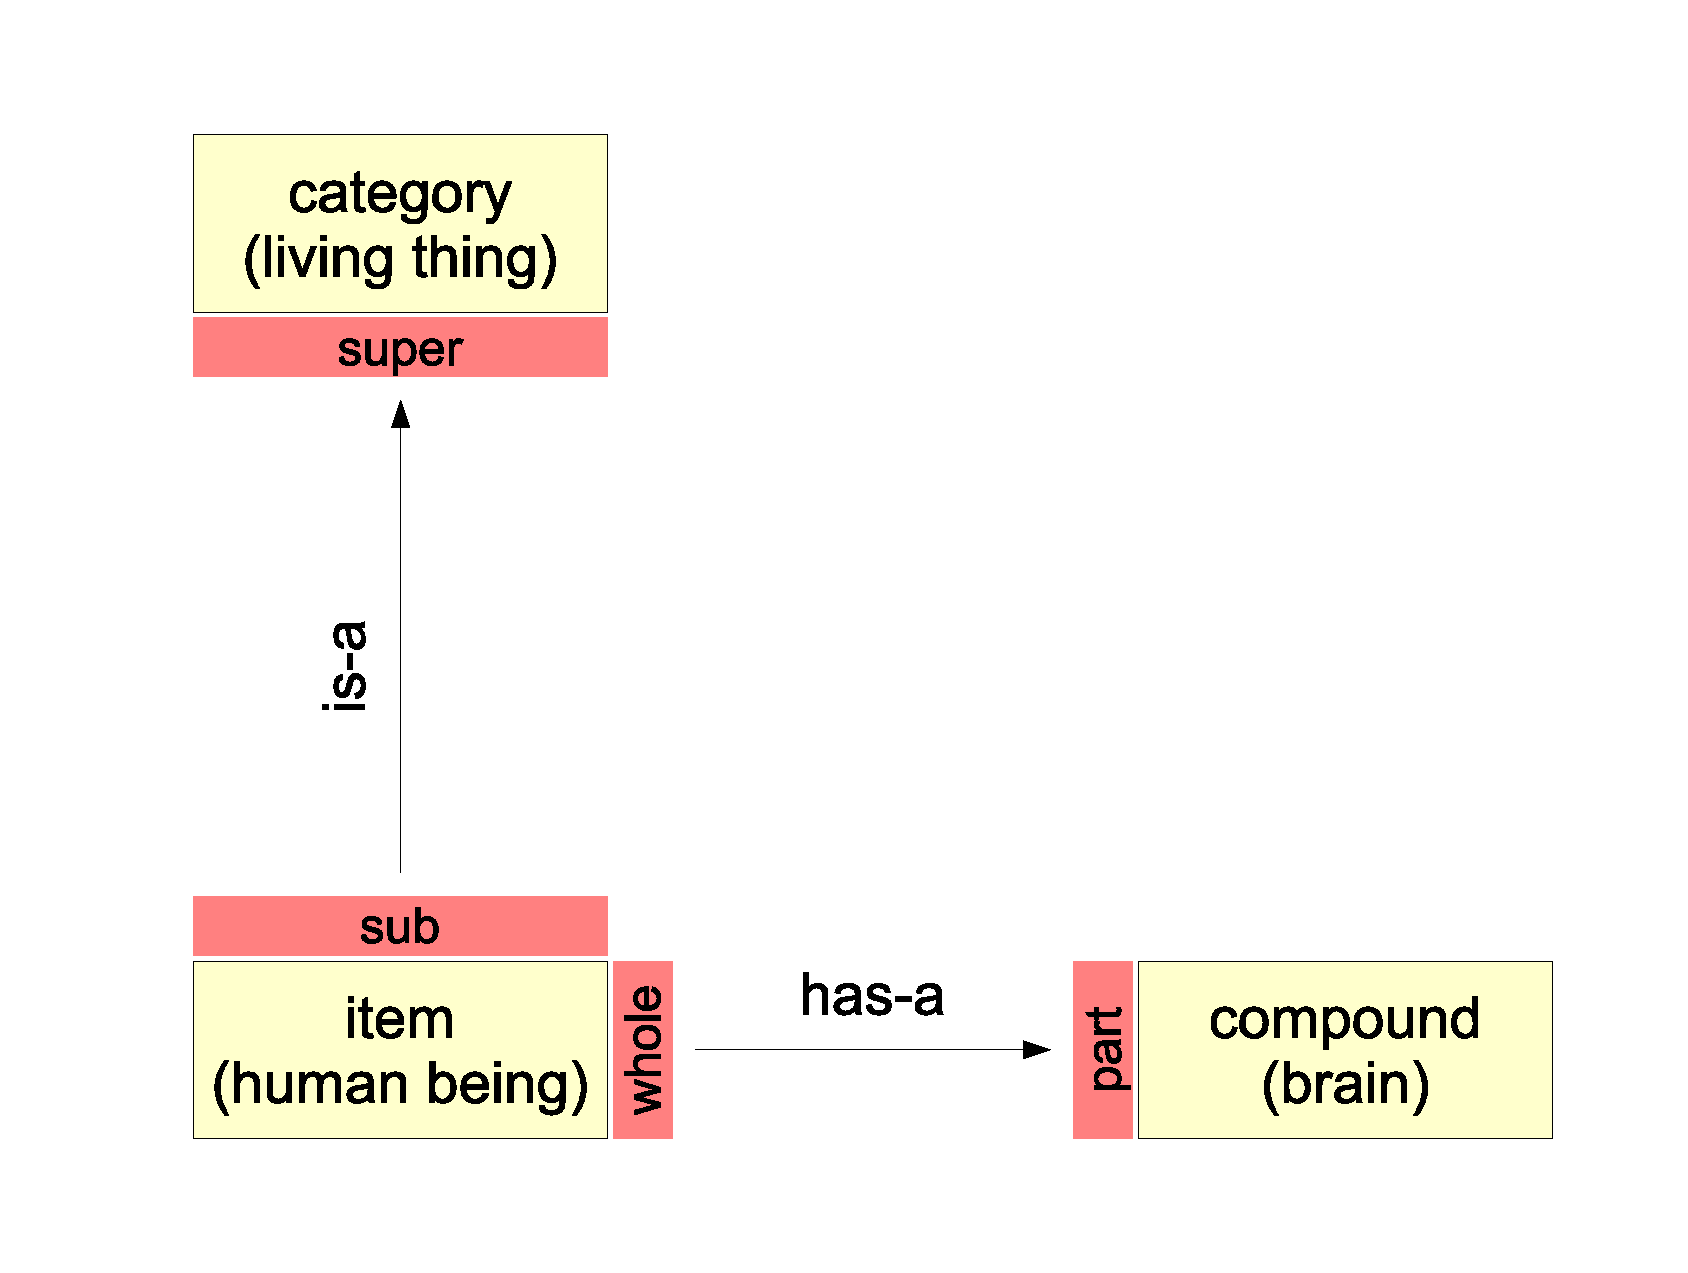
\includegraphics[scale=0.3]{vector/abstraction.eps}
        \caption{Abstractions of Human Thinking \cite{heller2004}}
        \label{abstraction_figure}
    \end{center}
\end{figure}

The latter two activities of abstraction -- categorization and composition --
are based on special \emph{Associations} (figure \ref{abstraction_figure}),
between a \emph{Super-} and a \emph{Sub} model and between a \emph{Whole-} and
a \emph{Part} model, respectively.

%
% $RCSfile: categories.tex,v $
%
% Copyright (c) 2004. Christian Heller. All rights reserved.
%
% No copying, altering, distribution or any other actions concerning this
% document, except after explicit permission by the author!
% At some later point in time, this document is planned to be put under
% the GNU FDL license. For now, _everything_ is _restricted_ by the author.
%
% http://www.cybop.net
% - Cybernetics Oriented Programming -
%
% http://www.resmedicinae.org
% - Information in Medicine -
%
% @author Christian Heller <christian.heller@tuxtax.de>
%

\subsection{Categories}
\label{categories_heading}

Most patterns heavily rely on associations, too. This paper therefore suggests to:

\begin{center}
    \textbf{Take the Kind of Association as Criterion\\
    to sort patterns in a completely new way.}
\end{center}

The opposite table shows a systematics of the new pattern categories with their
equivalents in human thinking, some representative example patterns and a
recommendation for their usage in software engineering. Patterns matching into
more than one category are placed after the priority: \emph{Recursion} over
\emph{Polymorphism}.

\begin{table}[ht]
    \begin{center}
        \begin{tabular}{| p{22mm} | p{20mm} | p{23mm} | p{10mm} |}
            \hline
            \textbf{Category} & \textbf{Equivalent} & \textbf{Representative} & \textbf{Advice}\\
            \hline
            Itemization & Discrimination & Command, Data Transfer Object, State, Memento, Envelope-Letter, Prototype & :-)\\
            \hline
            1:1 Association & Composition & Delegator, Object Adapter, Proxy (Surrogat, Client-/Server Stub), Wrapper, Handle-Body, Bridge & :-)\\
            \hline
            1:n Association & Composition & Whole-Part, View Handler, Broker (Mediator), Master-Slave, Command Processor, Counted Pointer, Chain of Responsibility & :-)\\
            \hline
            Recursion & Composition & Composite, Interpreter, Decorator, Linked Wrapper & :-)\\
            \hline
            Bidirectionalism & -- & Observer (Callback, Publisher-Subscriber), Forwarder-Receiver, Chain of Responsibility, Visitor, Reflection & :-(\\
            \hline
            Polymorphism & Categorization & Template Method, Builder, Factory Method, Class Adapter, Abstract Factory (Kit), Strategy (Validator, Policy), Iterator (Cursor) & :-$\mid$\\
            \hline
            Grouping & Categorization & Layers, Domain Model, MVC & :-)\\
            \hline
            Global Access & -- & Singleton, Flyweight, Registry, Manager & :-(\\
            \hline
        \end{tabular}
%        \caption{Pattern Systematics}
        \label{pattern_systematics_table}
    \end{center}
\end{table}

%
% $RCSfile: recommendation.tex,v $
%
% Copyright (c) 2004. Christian Heller. All rights reserved.
%
% No copying, altering, distribution or any other actions concerning this
% document, except after explicit permission by the author!
% At some later point in time, this document is planned to be put under
% the GNU FDL license. For now, _everything_ is _restricted_ by the author.
%
% http://www.cybop.net
% - Cybernetics Oriented Programming -
%
% http://www.resmedicinae.org
% - Information in Medicine -
%
% @author Christian Heller <christian.heller@tuxtax.de>
%

\subsection{Recommendation}
\label{recommendation_heading}

The first category \emph{Itemization} (objectification) is the base of any
modelling activity and clearly necessary.

The next three categories \emph{1:1 Association}, \emph{1:n Association} and
\emph{Recursion} are special kinds of associations that rely exclusively on
\emph{unidirectional} relations and result in a clean architecture which is why
their usage is strongly recommended.

\emph{Bidirectionalism}, on the other hand, is an \emph{ill} variant of the three
aforementioned categories and should be avoided wherever possible. Patterns in
this category are one reason for endless loops and unpredictable behaviour since
it becomes very difficult to trace the effects that changes in one place of a
system have on others (section \ref{bidirectional_dependency_heading}).

\emph{Polymorphism} is a good thing. It relies on categorization and due to
inheritance can avoid a tremendous amount of otherwise redundant source code.
However, it also makes understanding a system more difficult, since the whole
architecture must be understood before being able to manipulate code correctly.
Unwanted source code changes caused by inheritance dependencies are often
described with the term \emph{Fragile Base Class Problem}
\cite[section \emph{Layers}]{buschmann}. They are just the opposite of what
inheritance was actually intended to be for: \emph{Reusability}
\cite[Vorwort]{gruhn}.

\emph{Grouping} models is essential to keep overview in a complex software
system. A very promising technology to support this are \emph{Ontologies}
\cite{hellerkunze}. A lot of thought-work has to go into them but if they are
well thought-out, they are clearly recommended.

The habit of globally accessing models is banned since OOP became popular.
However, it is not banned completely. Patterns like \emph{Singleton}
encapsulate and bundle global access but they still permit it. They disregard
any dependencies and relations in a system, such are a security risk and reason
for untraceable data changes. This paper sees the whole category of
\emph{Global Access} as potentially dangerous and can \emph{not} recommend its
patterns.


    %
% $RCSfile: summary.tex,v $
%
% Copyright (c) 2001-2004. Christian Heller. All rights reserved.
%
% Permission is granted to copy, distribute and/or modify this document
% under the terms of the GNU Free Documentation License, Version 1.1
% or any later version published by the Free Software Foundation;
% with no Invariant Sections, with no Front-Cover Texts and with no Back-Cover
% Texts. A copy of the license is included in the section entitled
% "GNU Free Documentation License".
%
% http://www.cybop.net
% - Cybernetics Oriented Programming -
%
% http://www.resmedicinae.org
% - Information in Medicine -
%
% @author Christian Heller <christian.heller@tuxtax.de>
% @author Jens Bohl <info@jens-bohl.de>
%

\section{Summary}
\label{summary_heading}

Software design patterns are essential elements of frameworks. They can be
combined to comprise their advantages and to realize hierarchical structures.
These structures can be created and destroyed in the lifecycle of components.
In that lifecycle, object relations become more transparent and are easier to
control and to maintain.\\
Ontologies can help to model particular domains and to layer software. Every level
of these ontologies has a particular supertype, whereby these types depend on each
other by inheritance. This concept supports the modelling and logical separation
of software into hierarchical architectures. The granularity of the ontology
(number of ontological levels) can be adapted to particular requests.\\
By applying the new concepts introduced in this document, the quality of software
can be greatly increased. The time for building systems can be reduced to a minimum.
The clear architecture avoids common confusion as the systems grow.


    \label{references_heading}
    \bibliographystyle{plain}
    \bibliography{references}
\end{document}
